\documentclass[10pt,twocolumn,letterpaper]{article}
\usepackage{icl_eee_cw}
\usepackage{times}
\usepackage{epsfig}
\usepackage{graphicx}
\usepackage{amsmath}
\usepackage{amssymb}

\usepackage{courier}
\usepackage{color}

% Include other packages here, before hyperref.

% If you comment hyperref and then uncomment it, you should delete
% egpaper.aux before re-running latex.  (Or just hit 'q' on the first latex
% run, let it finish, and you should be clear).
\usepackage[breaklinks=true,bookmarks=false]{hyperref}

\cvprfinalcopy % *** Uncomment this line for the final submission

\def\cvprPaperID{****} % *** Enter the CVPR Paper ID here
\def\httilde{\mbox{\tt\raisebox{-.5ex}{\symbol{126}}}}

% Pages are numbered in submission mode, and unnumbered in camera-ready
%\ifcvprfinal\pagestyle{empty}\fi
\setcounter{page}{1}
\begin{document}




%%%%%%%%% TITLE
\title{Computer Vision and Pattern Recognition Coursework 1}
\author{TimZ}
\maketitle
%\thispagestyle{empty}
%\vspace{-5cm}




%%%%%%%%% BODY TEXT
%%%%%%%%% 1
\section{Collect Data}
\noindent The collected data are shown in the Appendix.




%%%%%%%%% 2
\section{Keypoints Correspondences}
\paragraph{2.1 Manual}
The Matlab function \texttt{\textcolor[RGB]{28,172,0}{ginput()}} is used in manually matching corresponding points, which returns the location of a clicked point on the image. Images are enlarged before clicking to generate relatively precise corresponding points. The result containing 10 pairs of keypoints is shown in Figure~\ref{fig:1}.
\begin{figure}[h]
\begin{center}  
   \includegraphics[width=0.47\textwidth]{2.1Manual}
\end{center}
   \caption{Manually Find Keypoints Correspondences}
\label{fig:1}
\end{figure}

\begin{figure}[h]
\begin{center}
   \includegraphics[width=0.47\textwidth]{2.2Automatic}
\end{center}
   \caption{Automatically Find Keypoints Correspondences}
\label{fig:2}
\end{figure}

\paragraph{2.2 Automatic}
After converting images to grayscale, the Harris Corner Detection algorithm is used to detect features (\texttt{\textcolor[RGB]{28,172,0}{detectHarrisFeatures()}}). This algorithm uses a local window to find areas where gray level changes rapidly and considers them as corner points. Then, the extracted features, also called descriptors, are derived according to these corner points using Matlab function \texttt{\textcolor[RGB]{28,172,0}{extractFeatures()}}. These descriptors are matched using function \texttt{\textcolor[RGB]{28,172,0}{matchFeatures()}} and reordered as matched points. The result is shown in Figure~\ref{fig:2}.


\paragraph{2.3 Comparison}
In Table~\ref{tab:1}, the quantity and correctness of correspondences are shown. The correctness of the 10 pairs of points chosen in Section 2.1 is verified by the function \texttt{\textcolor[RGB]{28,172,0}{estimateGeometricTransform2D()}} which considers all the 10 pairs of points as inliers. This function will be talked in Section 4.1 later. The automatic method is executed 50 times to find the average. It constantly returns 34 pairs of points, 23 pairs are correct in the best case, and 19 pairs are correct in the worst case.

\begin{table}[h]
\small
    \centering
    \begin{tabular}{c|c|c}
        Method & Quantity & {Correctness} \\
        \hline
        Manual & 10 & 100\% \\ 
        \hline
        Automatic (best) & 34 & 67.6\% \\ 
        \hline
        Automatic (Average) & 34 & 63.2\% \\ 
        \hline
        Automatic (worst)  & 34 & 55.9\% \\ 
    \end{tabular}%
    \medbreak
    \caption{Quantity and Correctness of the two Methods}
    \label{tab:1}
\end{table}

\noindent The result shows that finding keypoints correspondences manually is more accurate than automatically. It is obvious in Figure~\ref{fig:2} that some correspondences are incorrect. In terms of quantity, it is much faster and more convenient to use the automatic method to generate a large set of keypoints correspondences. Under the cost of correctness, the large quantity increases the robustness which also leads to the more accurate estimation of transformation.




%%%%%%%%% 3
\section{Camera Calibration}

\paragraph{3.1 Camera Parameters}
This section is performed by using the Camera Calibrator App in Matlab. 12 images are analysed and 4 of them have large reprojection errors, hence the remaining 8 images contribute to the result. The size of the checkerboard square is 28mm. With this parameter, the real-world coordinates of intersection points are known, and the intrinsic and extrinsic parameters are estimated. The camera-centric view is shown in Figure~\ref{fig:3}.
\begin{figure}[h]
\begin{center}
   \includegraphics[width=0.30\textwidth]{3.1}
\end{center}
   \caption{Camera-centric View}
\label{fig:3}
\end{figure}

\noindent The intrinsic matrix is shown bellow.
$$A=\begin{bmatrix}
465.587 & 0 & 0\\ 
-0.549 & 465.754 & 0\\ 
308.849 & 221.169 & 1
\end{bmatrix}$$
From the intrinsic matrix, the focal length is around 465.587 and 465.754, principle points locates at [308.849, 221.169], and the skew is -0.549. Other parameters and corresponding images are shown in the Appendix.


\paragraph{3.2 Distortions of Camera}
Distortions obtained from the Camera Calibrator App are shown in Table~\ref{tab:2}.
\begin{table}[h]
\small
    \centering
    \begin{tabular}{c|c}
        Radial Distortion & [0.134, -0.351]\\
        \hline
        Tangential Distortion & [-0.00343, 0.00377]\\ 
    \end{tabular}%
    \medbreak
    \caption{Estimated Distortions}
    \label{tab:2}
\end{table}

\noindent The result of the distortions are small, and there are no chromatic and spherical aberration. The main reason is that the modern mobile phone processes the taken images.




%%%%%%%%% 4
\section{Transformation Estimation}

\paragraph{4.1 Homography Matrix Estimation}
Using the automatic method in Section 2.2, 34 pairs of keypoints correspondences are inputted to the function \texttt{\textcolor[RGB]{28,172,0}{estimateGeometricTransform2D()}} with the \texttt{\textcolor[RGB]{170,4,249}{'projective'}} transform type. This function filters outliers in the keypoints correspondences using the M-estimator Sample Consensus (MSAC) algorithm. After filtering, 23 pairs of inliers remain, and the estimated homography matrix is shown below. From H, it can be found that the transformation type is projective with small rotation and translation, since the first two elements in the third row are large.
$$H=\begin{bmatrix} 
1.2728 & 0.0512 & 0.0001\\ 
-0.0345 & 1.2237 & -0.0000\\ 
-88.6485 & -60.3681 & 1.0000
\end{bmatrix}$$

\noindent The keypoints and their correspondences projected from the other image are shown in Figure~\ref{fig:4}.
\begin{figure}[h]
\begin{center}
    \includegraphics[width=0.47\textwidth]{4.1.png}
\end{center}
   \caption{Keypoints and Their Correspondences}
\label{fig:4}
\end{figure}


\paragraph{4.2.a Fundamental Matrix Estimation}
21 pairs of keypoints correspondences are found in 2 FD images. The function \texttt{\textcolor[RGB]{28,172,0}{estimateFundamentalMatrix()}} with method \texttt{\textcolor[RGB]{170,4,249}{'RANSAC'}} is used to compute the fundamental matrix. RANSAC is a robust estimation technique that can exclude outliers. Its limitation is that the results are not identical due to the randomness. 12 pairs of inliers remain after exclusion, and the estimated fundamental matrix is
$$ F=\begin{bmatrix}
-0.0000 & -0.0000 & 0.0171\\ 
0.0000 & -0.0000 & -0.0092\\ 
-0.0150 & 0.0056 & 0.9997
\end{bmatrix} $$
With the fundamental matrix and inliers, epipolar lines are found in Figure~\ref{fig:5} using the function \texttt{\textcolor[RGB]{28,172,0}{epipolarLine()}}. The intersection of epipolar lines is the epipole.

\begin{figure}[h]
\begin{center}
   \includegraphics[width=0.47\textwidth]{4.2}
\end{center}
   \caption{Keypoints and Their Corresponding Epipolar Lines}
\label{fig:5}
\end{figure}


\paragraph{4.2.b Vanishing Point and Horizon}
In order to clearly show the vanishing point and horizon, a special pair of images is taken. The vanishing point and horizon are found by the Hough Transform. Firstly, the edge of the image is detected by the function \texttt{\textcolor[RGB]{28,172,0}{edge()}} with the method \texttt{\textcolor[RGB]{170,4,249}{'canny'}}. Then, the functions \texttt{\textcolor[RGB]{28,172,0}{hough()}}, \texttt{\textcolor[RGB]{28,172,0}{houghpeaks()}}, and \texttt{\textcolor[RGB]{28,172,0}{houghlines()}} are used to detect the straight lines in the figure. Those straight lines are the yellow lines in Figure~\ref{fig:6}, and the intersection of the non-parallel yellow lines is the vanishing point (the cyan point). Originally, these non-parallel yellow lines should be parallel. They intersect due to the 3D view. The horizon should passing through the vanishing point, and since the remaining yellow lines are parallel, the horizon becomes the red line parallel to them.

\begin{figure}[h]
\begin{center}
   \includegraphics[width=0.27\textwidth]{4.2b}
\end{center}
   \caption{Vanishing Point and Horizon}
\label{fig:6}
\end{figure}




\paragraph{4.3 Tolerance of the Estimation Method to Outliers}
Similarly, \texttt{\textcolor[RGB]{28,172,0}{estimateFundamentalMatrix()}} is used. The method of it is set as \texttt{\textcolor[RGB]{170,4,249}{'RANSAC'}} with \texttt{\textcolor[RGB]{170,4,249}{'DistanceThreshold'}} being a large number (e.g. 10000) and \texttt{\textcolor[RGB]{170,4,249}{'Confidence'}} being 99.99, hence the algorithm considers all the matched points are inliers. The equation x'Fx is used to determine the correctness of estimated fundamental matrix. Theoretially, x'Fx = 0 for the correct fundamental matrix and keypoints correspondences.

\noindent Using the same two images as in Section 4.2, inputting different numbers of correct and incorrect keypoints correspondences, the result is shown in Table~\ref{tab:3}.

\begin{table}[h]
\small
    \centering
    \begin{tabular}{c|c|c|c}
        Correct & Incorrect & Correctness(\%) & Average x'Fx (e-04)\\
        \hline
        8 & 0 & 100 & -6.326\\ 
        \hline
        7 & 1 & 87.5 & -266.887\\ 
        \hline
        3 & 5 & 37.5 & 5248.640\\ 
        \hline
        8 & 1 & 88.9 & -79.695\\ 
        \hline
        8 & 5 & 61.5 & 277.603\\ 
        \hline
        16 & 0 & 100 & -6.138\\ 
        \hline
        16 & 1 & 94.1 & -12.254\\ 
        \hline
        16 & 5 & 76.2 & -50.653\\ 
    \end{tabular}%
    \medbreak
    \caption{Tolerance to Outliers}
    \label{tab:3}
\end{table}

\noindent In order to calculate the fundamental matrix, at least 8 pairs of keypoints correspondences are required. From the result, it is clear that the average x'Fx approaches to 0 as the increase of correct correspondences and the decrease of incorrect ones. However, the average x'Fx is related to but not determined by the correctness. Generally, the average x'Fx approaches to 0 as the increase of correctness, but if the number of correct correspondences is much larger, e.g. (8, 1) and (16, 5), this is not true. Therefore, the number of outliers this estimation method tolerates is determined both by the number of inliers and outliers.




%%%%%%%%% 5
\section{3D geometry}
\paragraph{5.1 Stereo Rectification} 
With the estimated fundamental matrix and the keypoints correspondences, the rectification matrix for each image is found by the function \texttt{\textcolor[RGB]{28,172,0}{estimateUncalibratedRectification()}}. Then, \texttt{\textcolor[RGB]{28,172,0}{rectifyStereoImages()}} takes the rectification matrices as input and rectifies the original images. Figure~\ref{fig:7} shows the original images and the result after stereo rectification.
\begin{figure}[h]
\begin{center}
   \includegraphics[width=0.47\textwidth]{5.10}
   \includegraphics[width=0.47\textwidth]{5.13}
\end{center}
   \caption{Stereo Rectification}
\label{fig:7}
\end{figure}

\noindent Obviously, the epipolar lines are parallel in the rectified images, since they are projected to a common plane. During the experiment, we found that in order to get a good result, the epipoles of the original images should be far from the images. This makes the projection to the common plane does not change the original images much. Therefore, we took these two images specially for this task. 


\paragraph{5.2 Depth Estimation} In order to obtain the depth map, the disparity map should be found. Firstly, using the function \texttt{\textcolor[RGB]{28,172,0}{stereoAnaglyph()}} to compute the stereo anaglyph of the rectified images (shown in Appendix) to determine the range of disparity. Then, the disparity map is obtained with the function \texttt{\textcolor[RGB]{28,172,0}{disparitySGM()}}, hence the depth map. It is clear in Figure~\ref{fig:8} that the depth of the closest box is the lowest, and the furthest areas are on the wall. The unit of measurement is centimetres.

\begin{figure}[h]
\begin{center}
   \includegraphics[width=0.27\textwidth]{5.21}
\end{center}
   \caption{Depth Map}
\label{fig:8}
\end{figure}

\clearpage

{\small
\bibliographystyle{ieee}
\bibliography{egbib}
[1] Krystian Mikolajczyk, Ad Spiers, Computer Vision and Pattern Recognition Lecture Slides.

\noindent [2] Harris, C., and M. Stephens, "A Combined Corner and Edge Detector," Proceedings of the 4th Alvey Vision Conference, August 1988, pp. 147-151.

\noindent [3] Hartley, R., A. Zisserman, Multiple View Geometry in Computer Vision, Cambridge University Press, 2003.

\noindent [4] Richard Szeliski, Computer Vision: Algorithms and Applications, 2nd ed., The University of Washington, Final draft 2021.
}


~\\

%%%%%%%%% A
\section*{Appendix}

\paragraph{1.}Collect Data

\noindent FD

\begin{figure}[h]
\begin{center}
   \includegraphics[width=0.46\textwidth]{FD}
\end{center}
\end{figure}


\noindent HG

\begin{figure}[h]
\begin{center}
   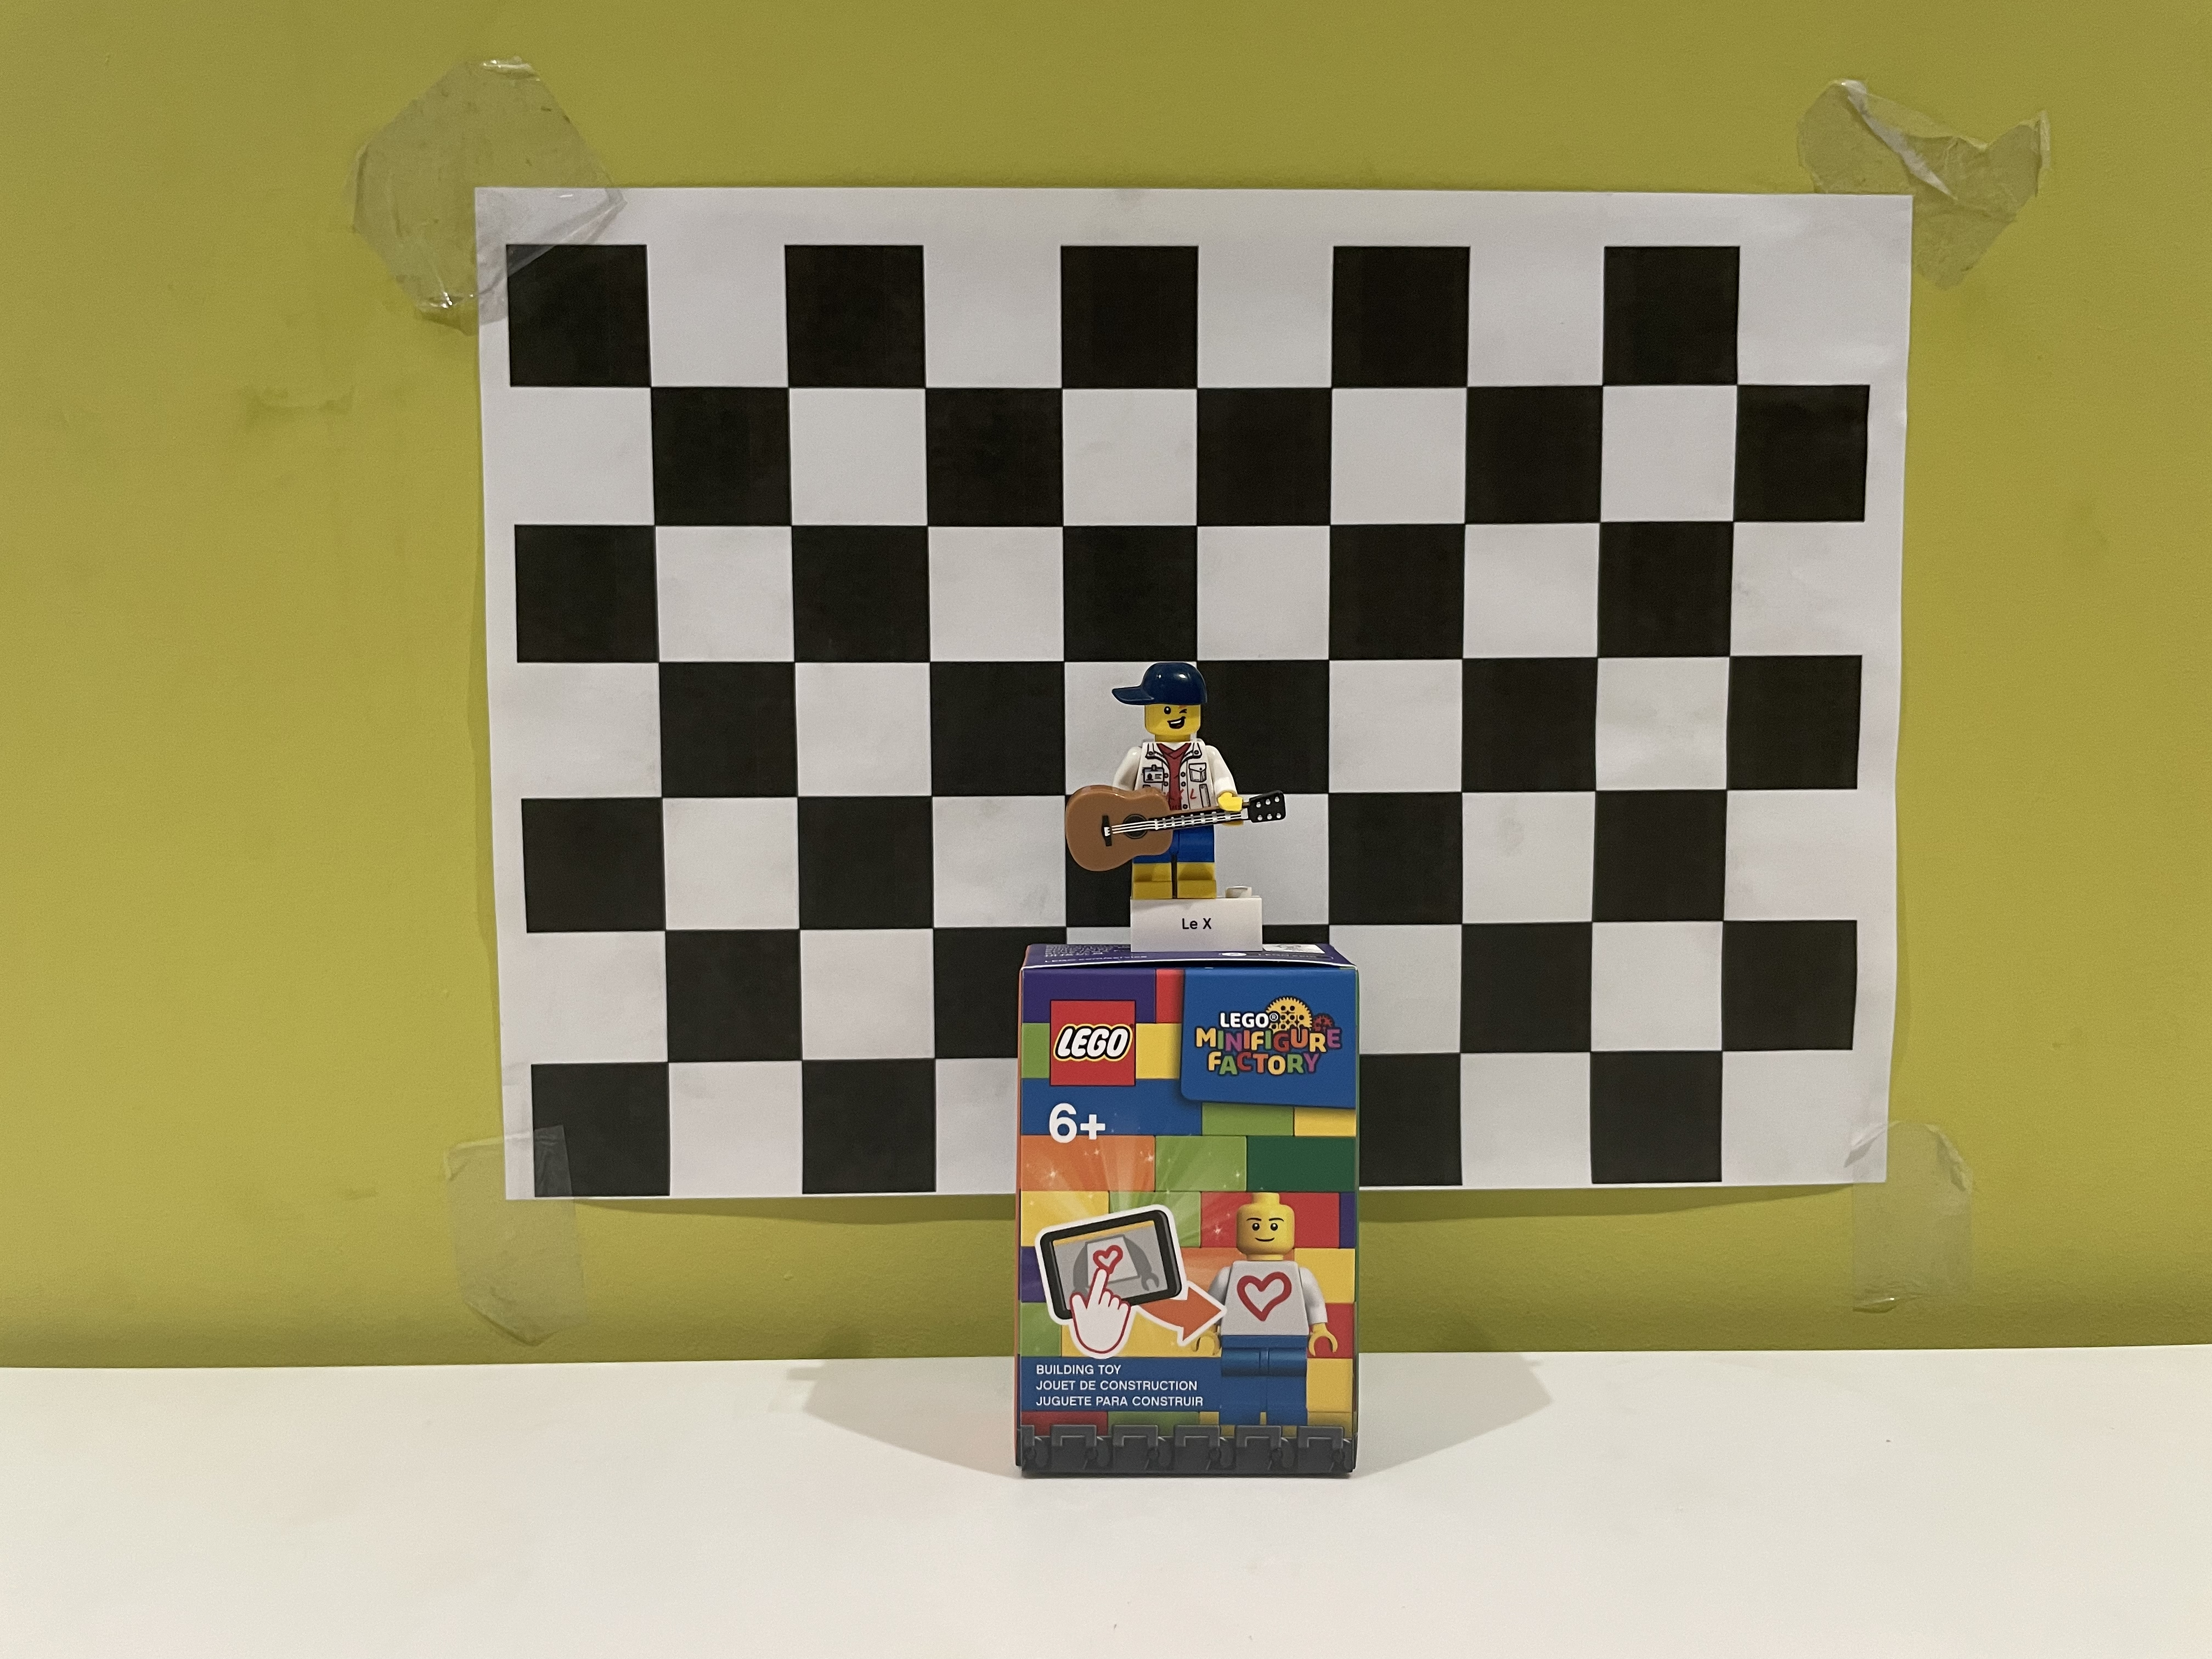
\includegraphics[width=0.47\textwidth]{HG1_ORI}
   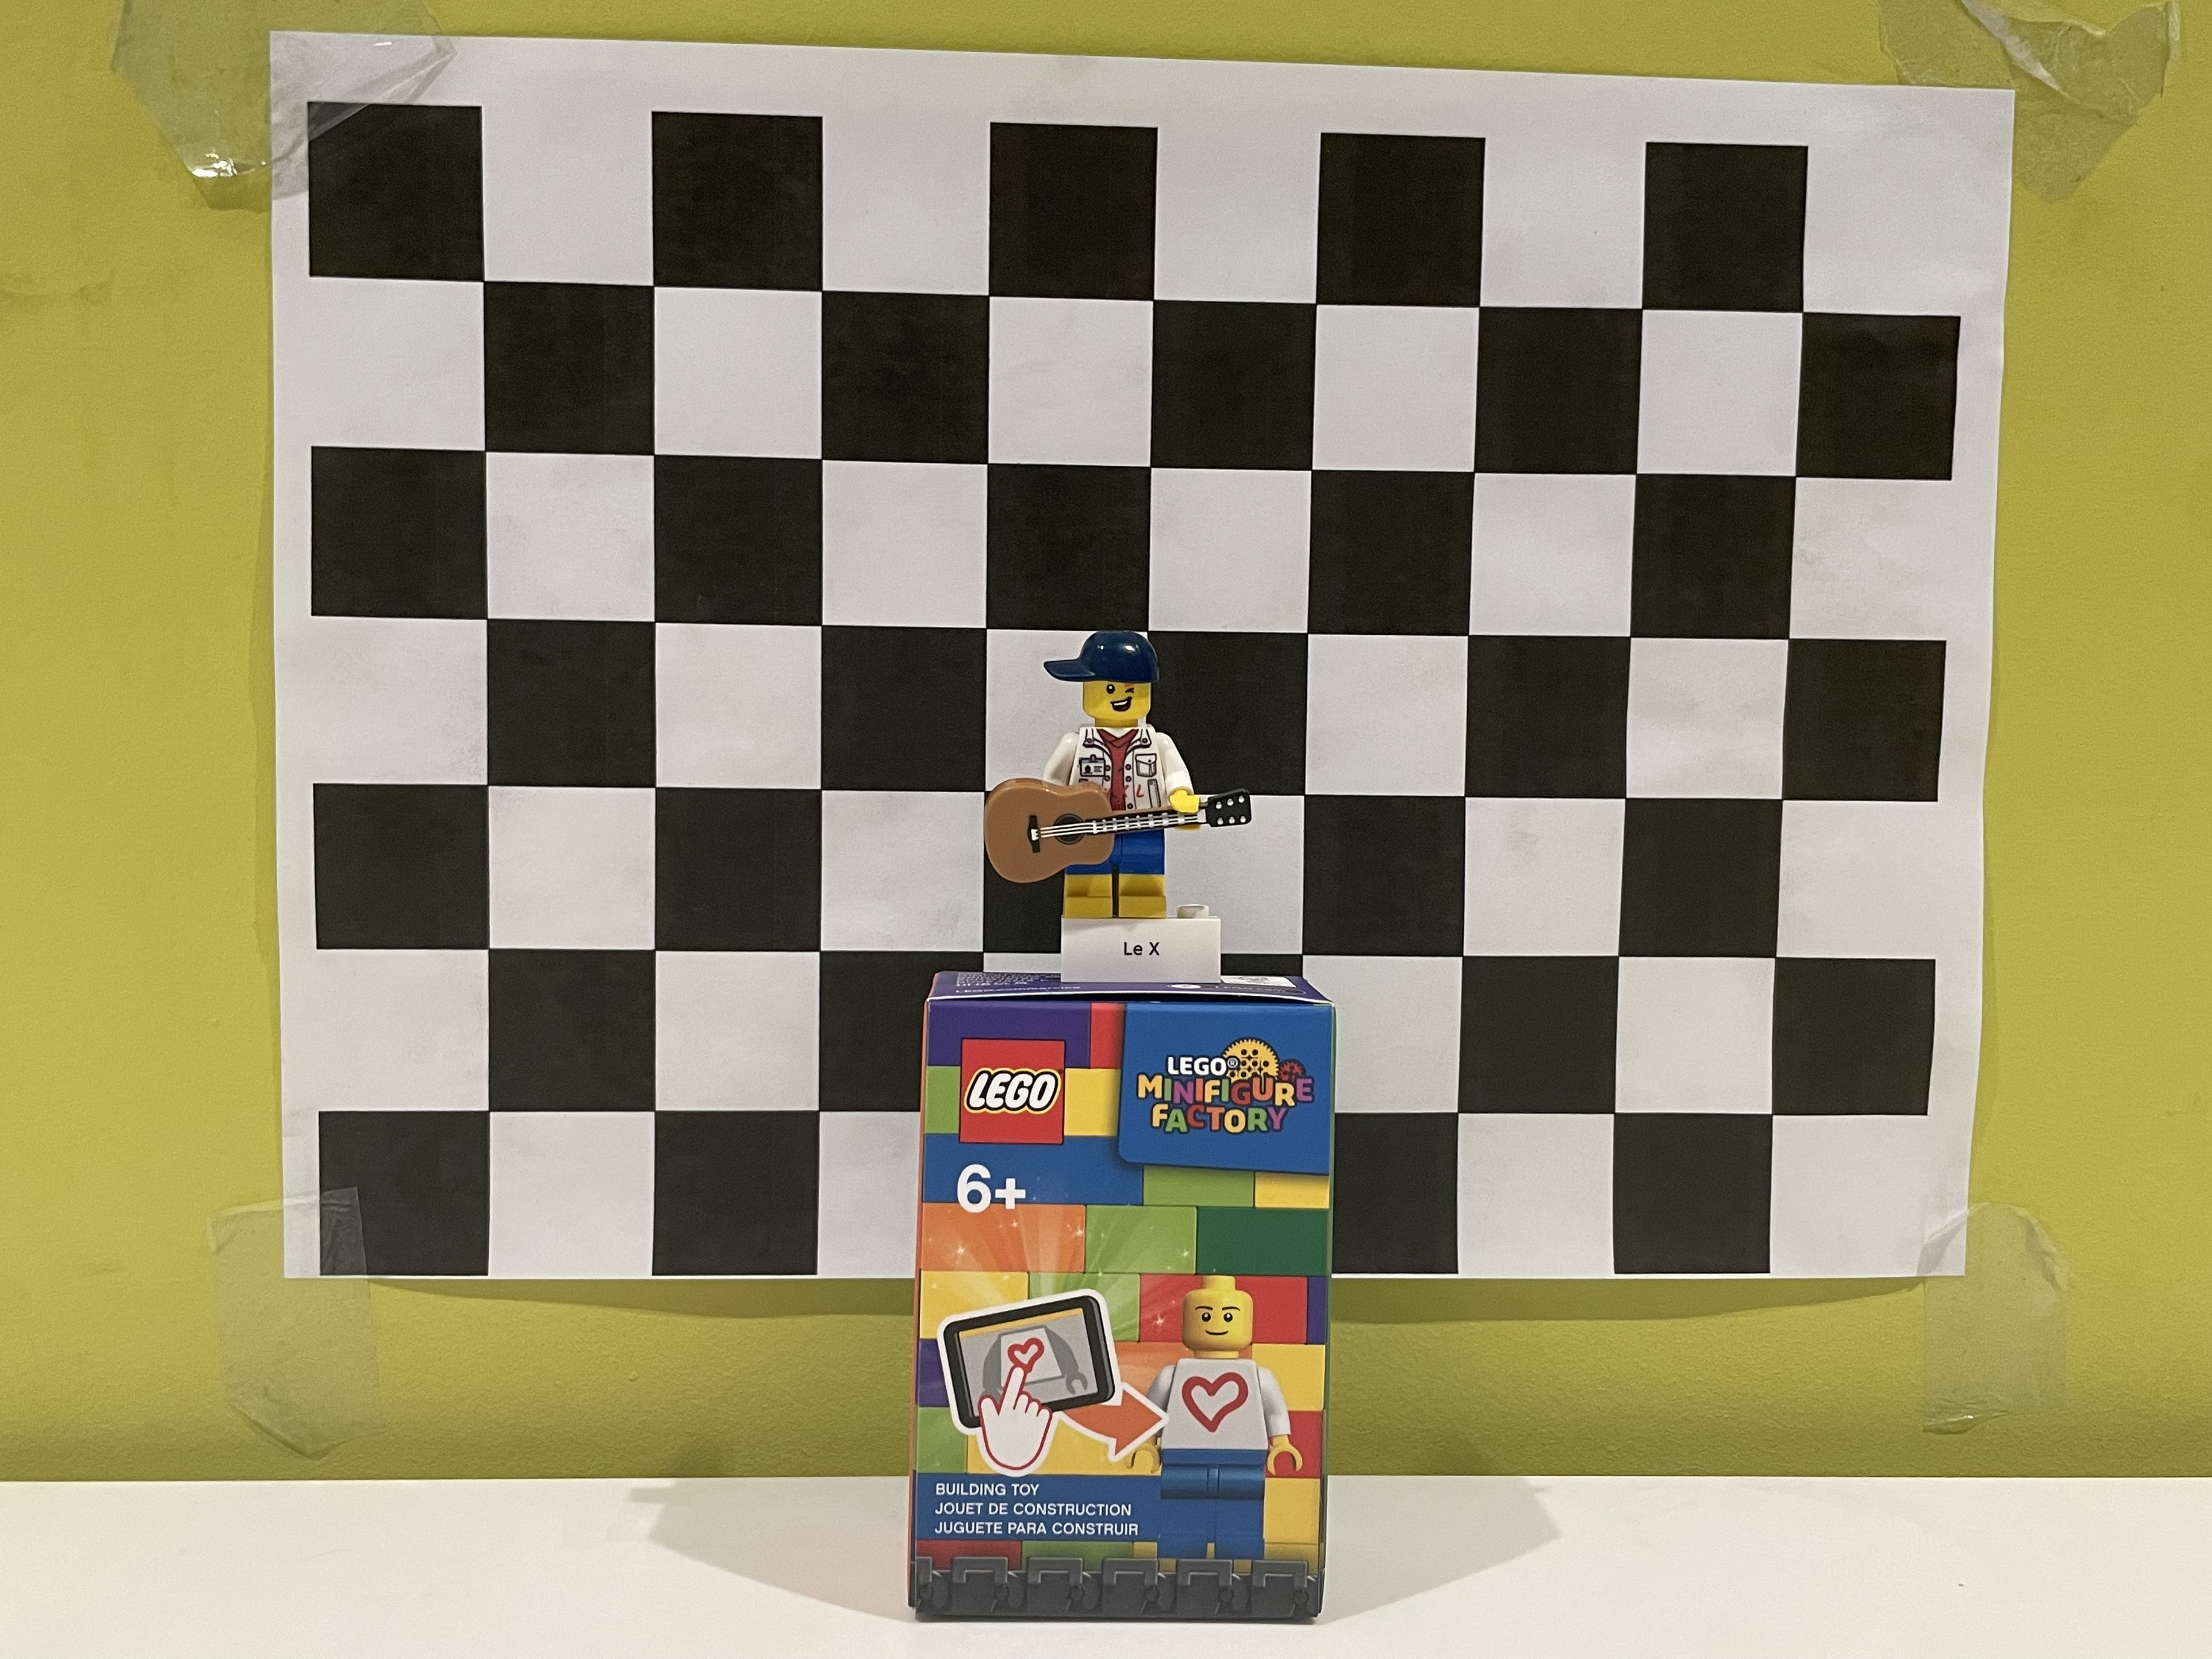
\includegraphics[width=0.47\textwidth]{HG1_X1.2+ROT RIGHT}
\end{center}
\end{figure}


\paragraph{3.}Camera Calibration

\begin{figure}[h]
\begin{center}
   \includegraphics[width=0.47\textwidth]{3.4}
\end{center}
\end{figure}

\begin{figure}[h]
\begin{center}
   \includegraphics[width=0.47\textwidth]{C3.0}
\end{center}
\end{figure}

\begin{figure}[h]
\begin{center}
   \includegraphics[width=0.47\textwidth]{3.3}
\end{center}
\end{figure}

\begin{figure}[h]
\begin{center}
   \includegraphics[width=0.47\textwidth]{3.2}
\end{center}
\end{figure}



\begin{table}[h]
\small
    \centering
    \begin{tabular}{c|c}
        Translation Vectors & 
        $\begin{bmatrix}
        -102.724 & -78.377 & 299.687 \\
        0.0000 & -0.0000 & -0.0092 \\
        -0.0150 & 0.0056 & 0.9997 \\
        -100.400&	-88.859	  &  316.653 \\
        -144.810&	-70.910	 &   367.874 \\
        -100.937&	-63.209	  &  295.231 \\
        -115.607&	-103.616&	367.274 \\
        -120.888&	-49.525	 &   389.973 \\
        -138.360&	-84.832	  &  342.053 \\
        -152.778&	-106.884&	432.160
        \end{bmatrix}$ \\
        \hline
        Translation Vectors Error   & 
        $\begin{bmatrix}
        0.615&	0.527&	1.466\\
        0.640&	0.543&	1.529\\
        0.724&	0.640&	1.718\\
        0.594&	0.502&	1.402\\
        0.752&	0.643&	1.796\\
        0.792&	0.682&	1.933\\
        0.712&	0.606&	1.723\\
        0.868&	0.756&	2.103
        \end{bmatrix}$ \\ 
        \hline
        Rotation Matrix 1 & 
        $\begin{bmatrix}
        0.9952  &  0.0108  &  0.0972\\
        -0.0203  &  0.9950 &   0.0974\\
        -0.0957  & -0.0989  &  0.9905
        \end{bmatrix}$ \\ 
        \hline
        Rotation Matrix 2 & 
        $\begin{bmatrix}
        0.9993 &  -0.0122  &  0.0358\\
        0.0139 &   0.9987 &  -0.0482\\
        -0.0351 &   0.0486  &  0.9982
        \end{bmatrix}$ \\ 
        \hline
        Rotation Matrix 3 & 
        $\begin{bmatrix}
    0.9835   & 0.0243  & -0.1791\\
   -0.0069  &  0.9952  &  0.0976\\
    0.1806  & -0.0947  &  0.9790
        \end{bmatrix}$ \\ 
        \hline
        Rotation Matrix 4 & 
        $\begin{bmatrix}
    0.9939  &  0.0419  &  0.1020\\
   -0.0259  &  0.9878  & -0.1533\\
   -0.1072  &  0.1497  &  0.9829
        \end{bmatrix}$ \\ 
        \hline
        Rotation Matrix 5 & 
        $\begin{bmatrix}
    0.9970  &  0.0050 &   0.0767\\
   -0.0088  &  0.9988 &   0.0491\\
   -0.0764  & -0.0497 &   0.9958
        \end{bmatrix}$ \\ 
        \hline
        Rotation Matrix 6 & 
        $\begin{bmatrix}
    0.9945  & -0.0092   & 0.1046\\
   -0.0164  &  0.9702 &   0.2418\\
   -0.1037  & -0.2422  &  0.9647
        \end{bmatrix}$ \\ 
        \hline
        Rotation Matrix 7 & 
        $\begin{bmatrix}
    0.9077  & -0.0331  &  0.4182\\
   -0.0189 &   0.9926  &  0.1197\\
   -0.4191  & -0.1166 &   0.9004
        \end{bmatrix}$ \\ 
        \hline
        Rotation Matrix 8 & 
        $\begin{bmatrix}
    0.9970  &  0.0441  & -0.0644\\
   -0.0373  &  0.9940  &  0.1031\\
    0.0685  & -0.1004  &  0.9926
        \end{bmatrix}$ \\ 
        \hline
                Rotation Vectors Error   & 
        $\begin{bmatrix}
0.00183 &	0.00192&	0.000255\\
0.00179&	0.00200&	0.000254\\
0.00196&	0.00224&	0.000338\\
0.00172&	0.00190&	0.000279\\
0.00234&	0.00212&	0.000289\\
0.00220&	0.00214&	0.000404\\
0.00206&	0.00219&	0.000479\\
0.00261&	0.00251&	0.000328
        \end{bmatrix}$ \\ 
    \end{tabular}%
    \medbreak
    \caption{Extrinsic Parameters}
\end{table}

\begin{table}[h]
\small
    \centering
    \begin{tabular}{c|c}
        Image Size & [454,605]\\ 
        \hline
        Mean Reprojection Error & 0.241\\ 
    \end{tabular}%
    \medbreak
    \caption{Other Camera Calibration Parameters}
\end{table}

\clearpage

\paragraph{5.}Stereo Anaglyph

\begin{figure}[h]
\begin{center}
   \includegraphics[width=0.46\textwidth]{5.20}
\end{center}
\end{figure}



\end{document}
